\section{DAPHNE Data Sample}

\hl{Aqui se agregaran las figuras de los datos y muestras que se tomaron en las pruebas de los AFEs, tanto de las senales generadas por los AFEs para ver la sincronizacion como de algunas muestras de senales reales generadas por generadores de senales y adquiridas por DAPHNE.}

\begin{figure}[htbp]
\centering % \begin{center}/\end{center} takes some additional vertical space
%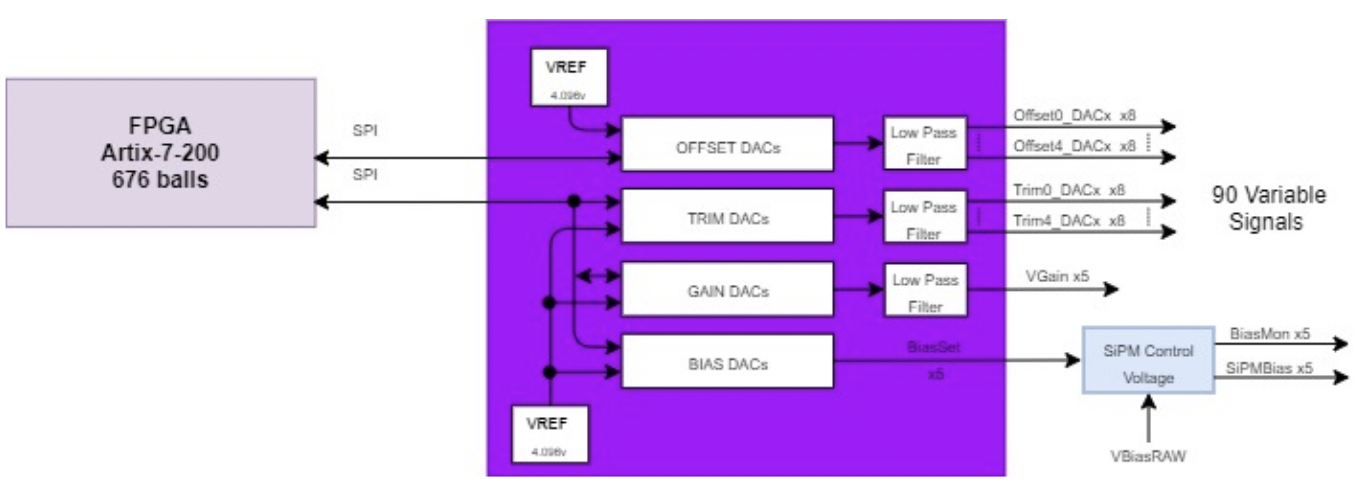
\includegraphics[width=.8\textwidth,trim=30 110 0 0,clip]{Images/BiasControl.png}
%\qquad
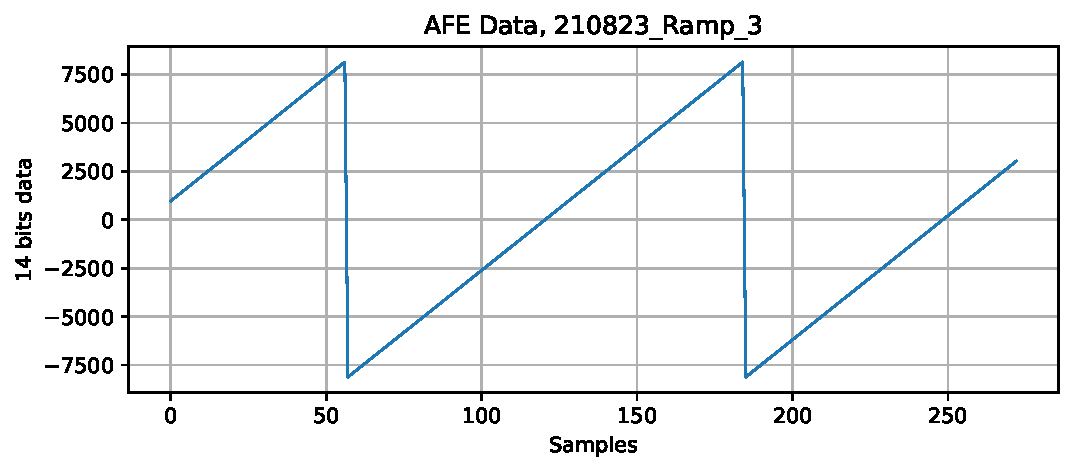
\includegraphics[width=0.9\textwidth,origin=c,angle=0]{Images/DaphneAFETest/210823_Ramp_3.pdf}
% "\includegraphics" from the "graphicx" permits to crop (trim+clip)
% and rotate (angle) and image (and much more)
\caption{\label{fig:InitPeriTask} Control and configuration task scheme.}
\end{figure}


\begin{figure}[htbp]
\centering % \begin{center}/\end{center} takes some additional vertical space
%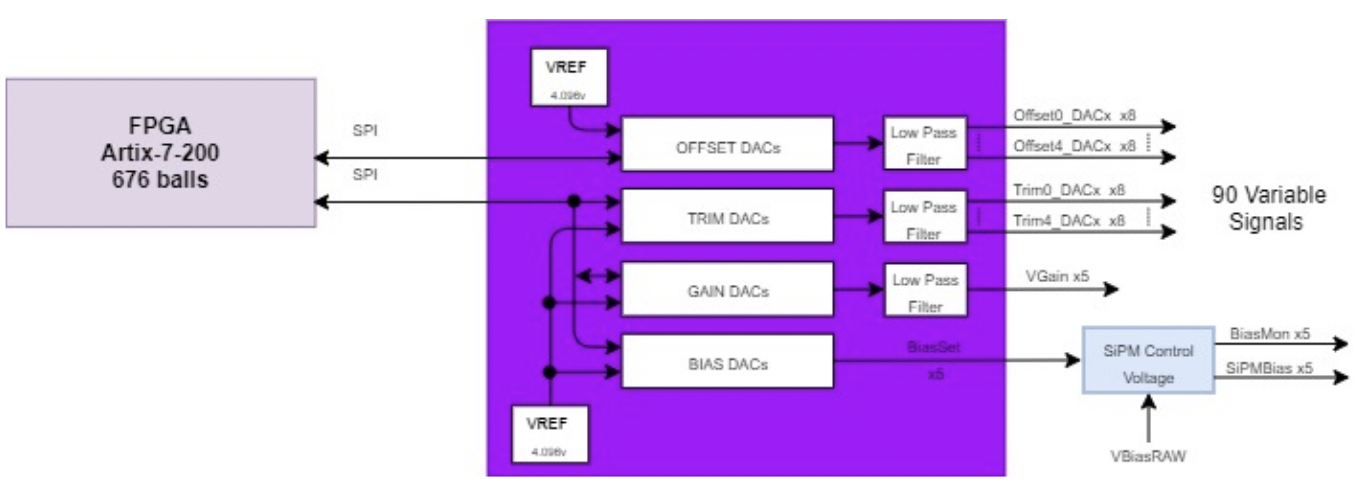
\includegraphics[width=.8\textwidth,trim=30 110 0 0,clip]{Images/BiasControl.png}
%\qquad
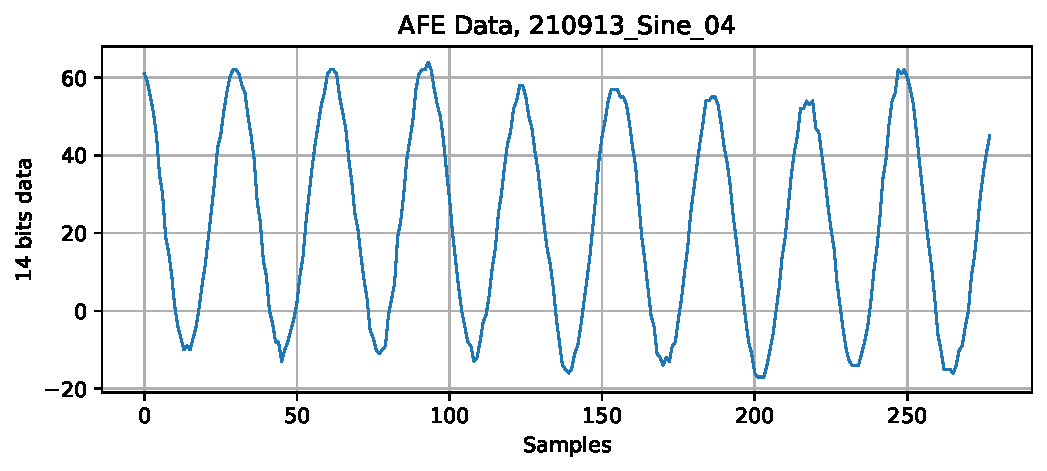
\includegraphics[width=0.9\textwidth,origin=c,angle=0]{Images/DaphneAFETest/210913_Sine_04.pdf}
% "\includegraphics" from the "graphicx" permits to crop (trim+clip)
% and rotate (angle) and image (and much more)
\caption{\label{fig:InitPeriTask} Control and configuration task scheme.}
\end{figure}


\begin{figure}[htbp]
\centering % \begin{center}/\end{center} takes some additional vertical space
%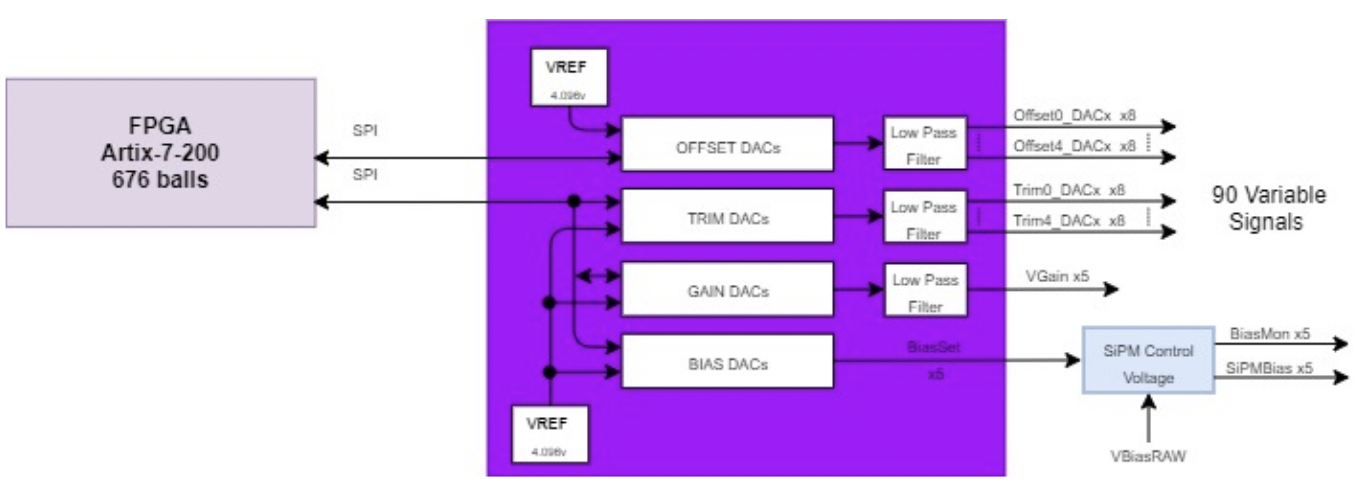
\includegraphics[width=.8\textwidth,trim=30 110 0 0,clip]{Images/BiasControl.png}
%\qquad
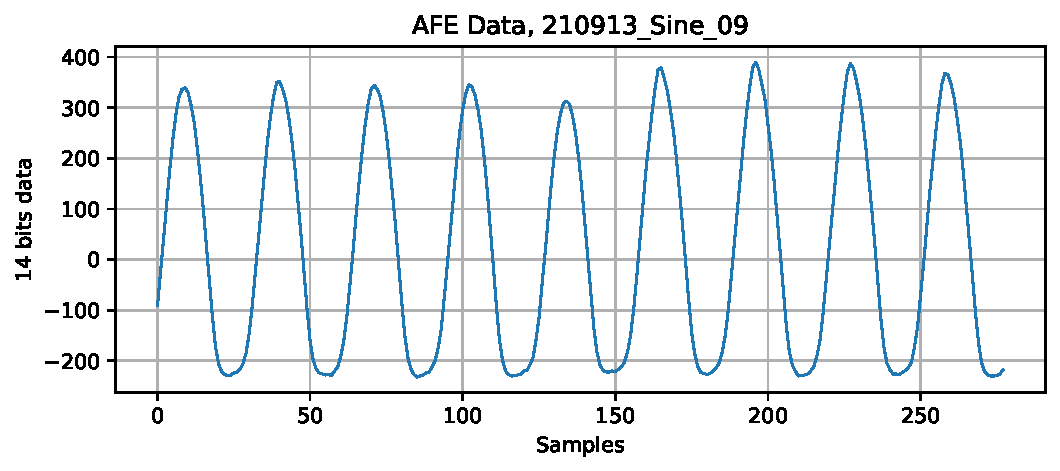
\includegraphics[width=0.9\textwidth,origin=c,angle=0]{Images/DaphneAFETest/210913_Sine_09.pdf}
% "\includegraphics" from the "graphicx" permits to crop (trim+clip)
% and rotate (angle) and image (and much more)
\caption{\label{fig:InitPeriTask} Control and configuration task scheme.}
\end{figure}



\begin{figure}[htbp]
\centering % \begin{center}/\end{center} takes some additional vertical space
%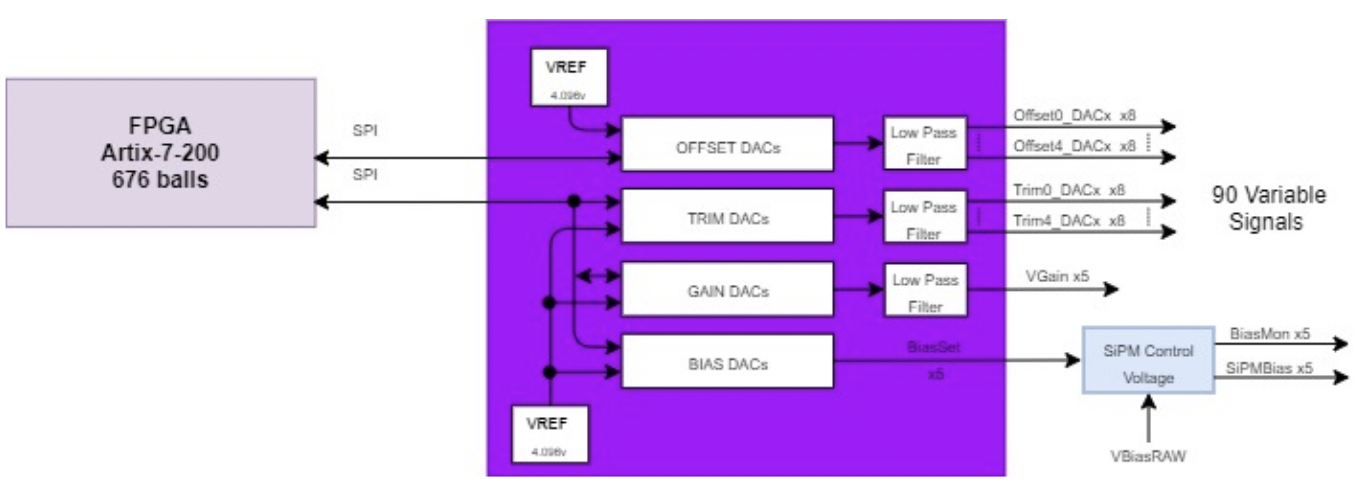
\includegraphics[width=.8\textwidth,trim=30 110 0 0,clip]{Images/BiasControl.png}
%\qquad
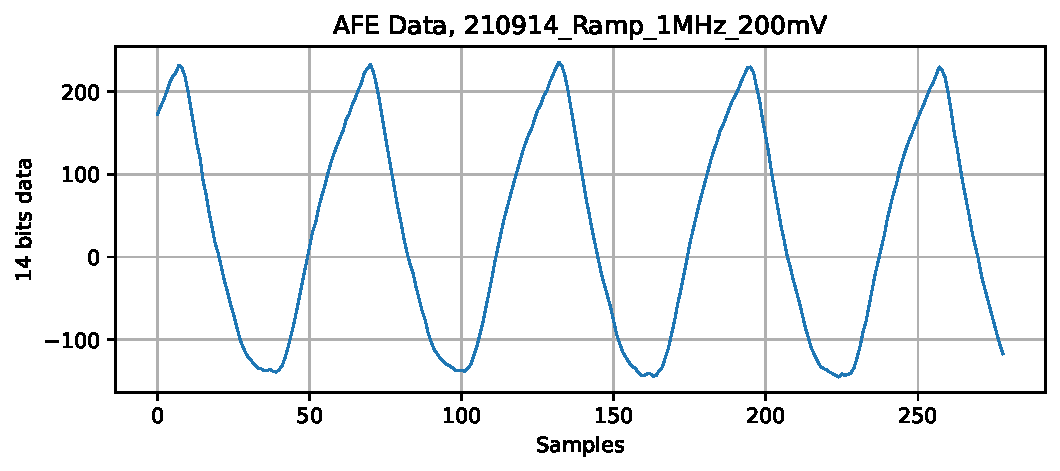
\includegraphics[width=0.9\textwidth,origin=c,angle=0]{Images/DaphneAFETest/210914_Ramp_1MHz_200mV.pdf}
% "\includegraphics" from the "graphicx" permits to crop (trim+clip)
% and rotate (angle) and image (and much more)
\caption{\label{fig:InitPeriTask} Control and configuration task scheme.}
\end{figure}

\begin{figure}[htbp]
\centering % \begin{center}/\end{center} takes some additional vertical space
%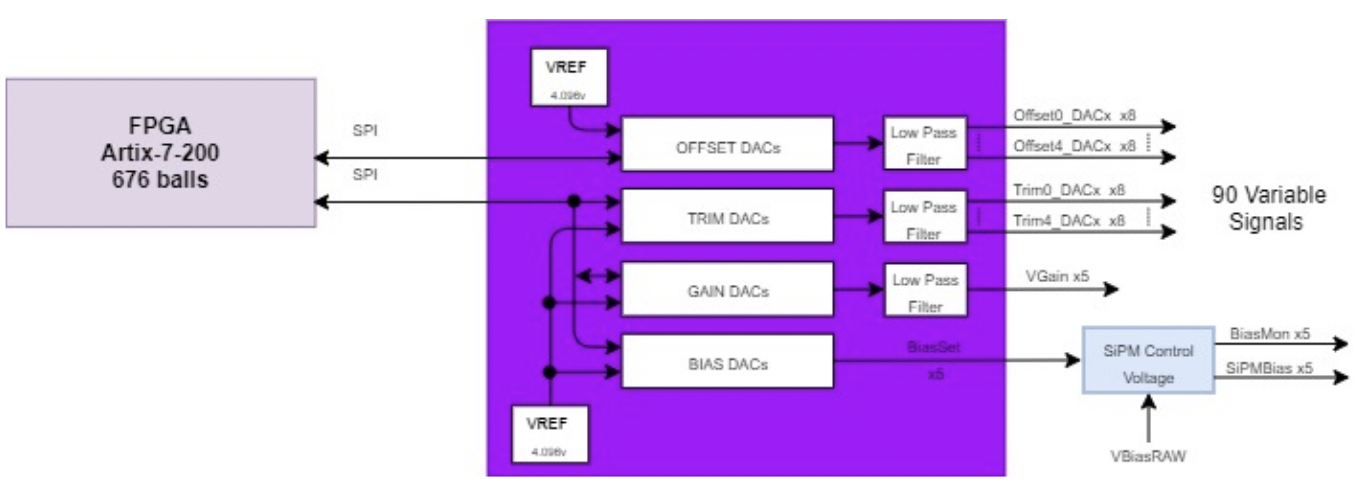
\includegraphics[width=.8\textwidth,trim=30 110 0 0,clip]{Images/BiasControl.png}
%\qquad
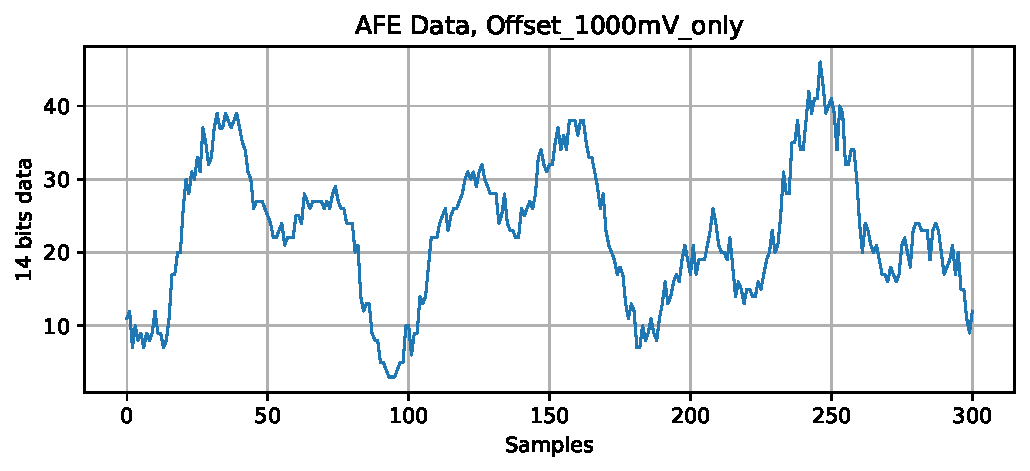
\includegraphics[width=0.9\textwidth,origin=c,angle=0]{Images/DaphneAFETest/Offset_1000mV_only.pdf}
% "\includegraphics" from the "graphicx" permits to crop (trim+clip)
% and rotate (angle) and image (and much more)
\caption{\label{fig:InitPeriTask} Control and configuration task scheme.}
\end{figure}


\begin{figure}[htbp]
\centering % \begin{center}/\end{center} takes some additional vertical space
%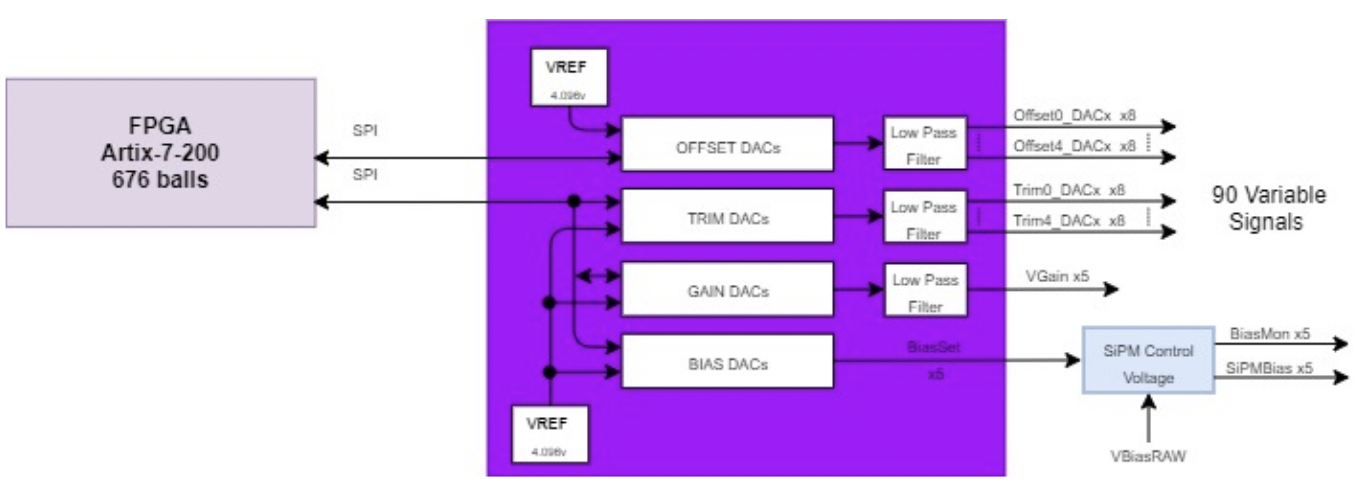
\includegraphics[width=.8\textwidth,trim=30 110 0 0,clip]{Images/BiasControl.png}
%\qquad
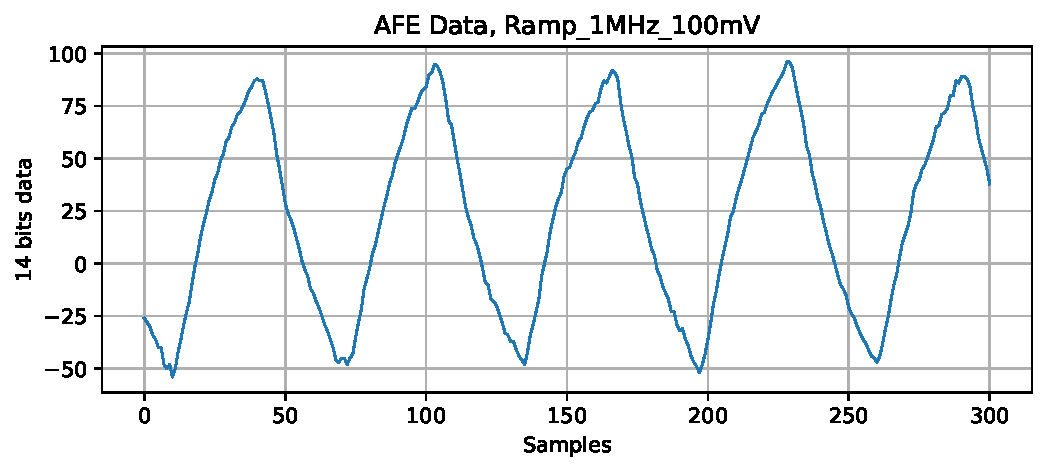
\includegraphics[width=0.9\textwidth,origin=c,angle=0]{Images/DaphneAFETest/Ramp_1MHz_100mV.pdf}
% "\includegraphics" from the "graphicx" permits to crop (trim+clip)
% and rotate (angle) and image (and much more)
\caption{\label{fig:InitPeriTask} Control and configuration task scheme.}
\end{figure}

\begin{figure}[htbp]
\centering % \begin{center}/\end{center} takes some additional vertical space
%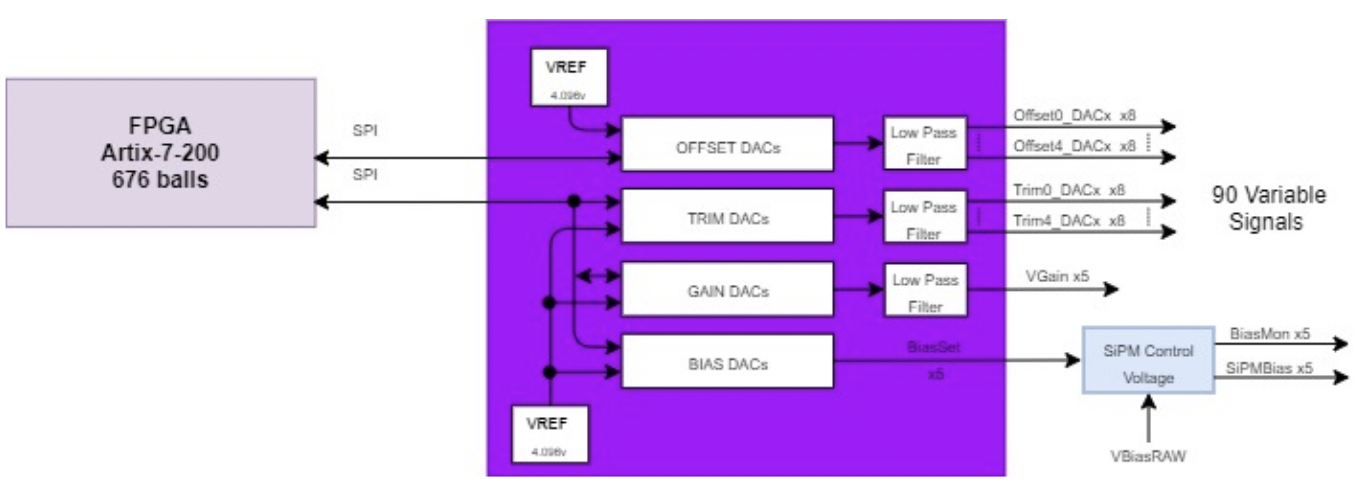
\includegraphics[width=.8\textwidth,trim=30 110 0 0,clip]{Images/BiasControl.png}
%\qquad
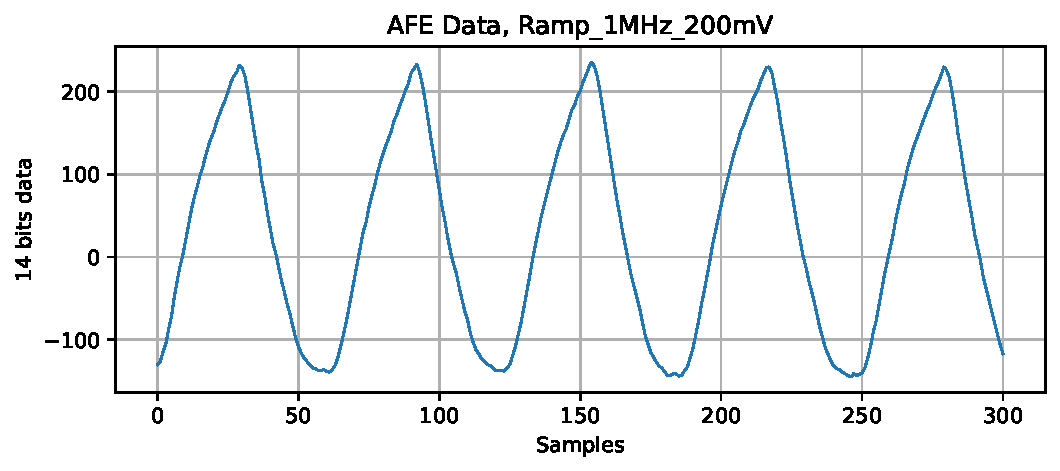
\includegraphics[width=0.9\textwidth,origin=c,angle=0]{Images/DaphneAFETest/Ramp_1MHz_200mV.pdf}
% "\includegraphics" from the "graphicx" permits to crop (trim+clip)
% and rotate (angle) and image (and much more)
\caption{\label{fig:InitPeriTask} Control and configuration task scheme.}
\end{figure} 
        

        

        